<tipo = seleccion unica, orden = aleatorio>

<pregunta>
Uno de los siguientes diagramas no puede ser doblado para formar un cubo. ¿Cuál de ellos?

<item>
\raisebox{-1ex}{
	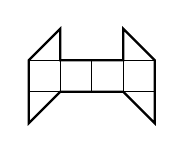
\begin{tikzpicture}[thin,scale=0.4]
		\draw [thick] (12,0) -- (13,1) -- (15,1) -- (16,0) -- (16,2) -- (15,3) -- (15,2) -- (13,2) -- (13,3) -- (12,2) -- cycle;
		\draw (12,2) -- (13,2) -- (13,1) -- (12,1);
		\draw (14,1) -- (14,2);
		\draw (16,2) -- (15,2) -- (15,1) -- (16,1);
  \end{tikzpicture}}
\bigskip
		
<item>
\raisebox{-1ex}{
	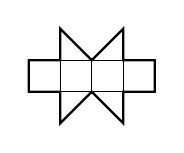
\begin{tikzpicture}[thin,scale=0.4]
		\draw [thick] (0,1) -- (1,1) -- (1,0) -- (2,1) -- (3,0) -- (3,1) -- (4,1) -- (4,2) -- (3,2) -- (3,3) -- (2,2) -- (1,3) -- (1,2) -- (0,2) -- cycle;
		\draw (1,1) rectangle (3,2);
		\draw (2,1) -- (2,2);
  \end{tikzpicture}}
\bigskip
		
<item>
\raisebox{-1ex}{
	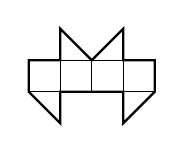
\begin{tikzpicture}[thin,scale=0.4]
		\draw [thick] (6,1) -- (7,0) -- (7,1) -- (9,1) -- (9,0) -- (10,1) -- (10,2) -- (9,2) -- (9,3) -- (8,2) -- (7,3) -- (7,2) -- (6,2) -- cycle;
		\draw (6,1) -- (7,1) -- (7,2) -- (8,2) -- (8,1);
		\draw (8,2) -- (9,2) -- (9,1) -- (10,1);
  \end{tikzpicture}}
\bigskip

<item>
\raisebox{-1ex}{
	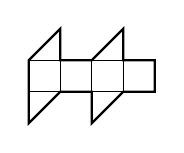
\begin{tikzpicture}[thin,scale=0.4]
		\draw [thick] (18,0) -- (19,1) -- (20,1) -- (20,0) -- (21,1) -- (22,1) -- (22,2) -- (21,2) -- (21,3) -- (20,2) -- (19,2) -- (19,3) -- (18,2) -- cycle;
		\draw (18,1) rectangle (19,2);
		\draw (20,1) rectangle (21,2);
  \end{tikzpicture}}
\bigskip

<item>
\raisebox{-1ex}{
	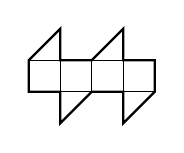
\begin{tikzpicture}[thin,scale=0.4]
		\draw [thick] (24,1) -- (25,1) -- (25,0) -- (26,1) -- (27,1) -- (27,0) -- (28,1) -- (28,2) -- (27,2) -- (27,3) -- (26,2) -- (25,2) -- (25,3) -- (24,2) -- cycle;
		\draw (24,2) -- (25,2) -- (25,1) -- (26,1) -- (26,2) -- (27,2) -- (27,1) -- (28,1);
  \end{tikzpicture}}
\bigskip

